\documentclass[../main.tex]{subfiles}

\begin{document}
\begin{figure}[H]
	\centering
	\caption{A picture showing the differences in the same map from Diablo III}
	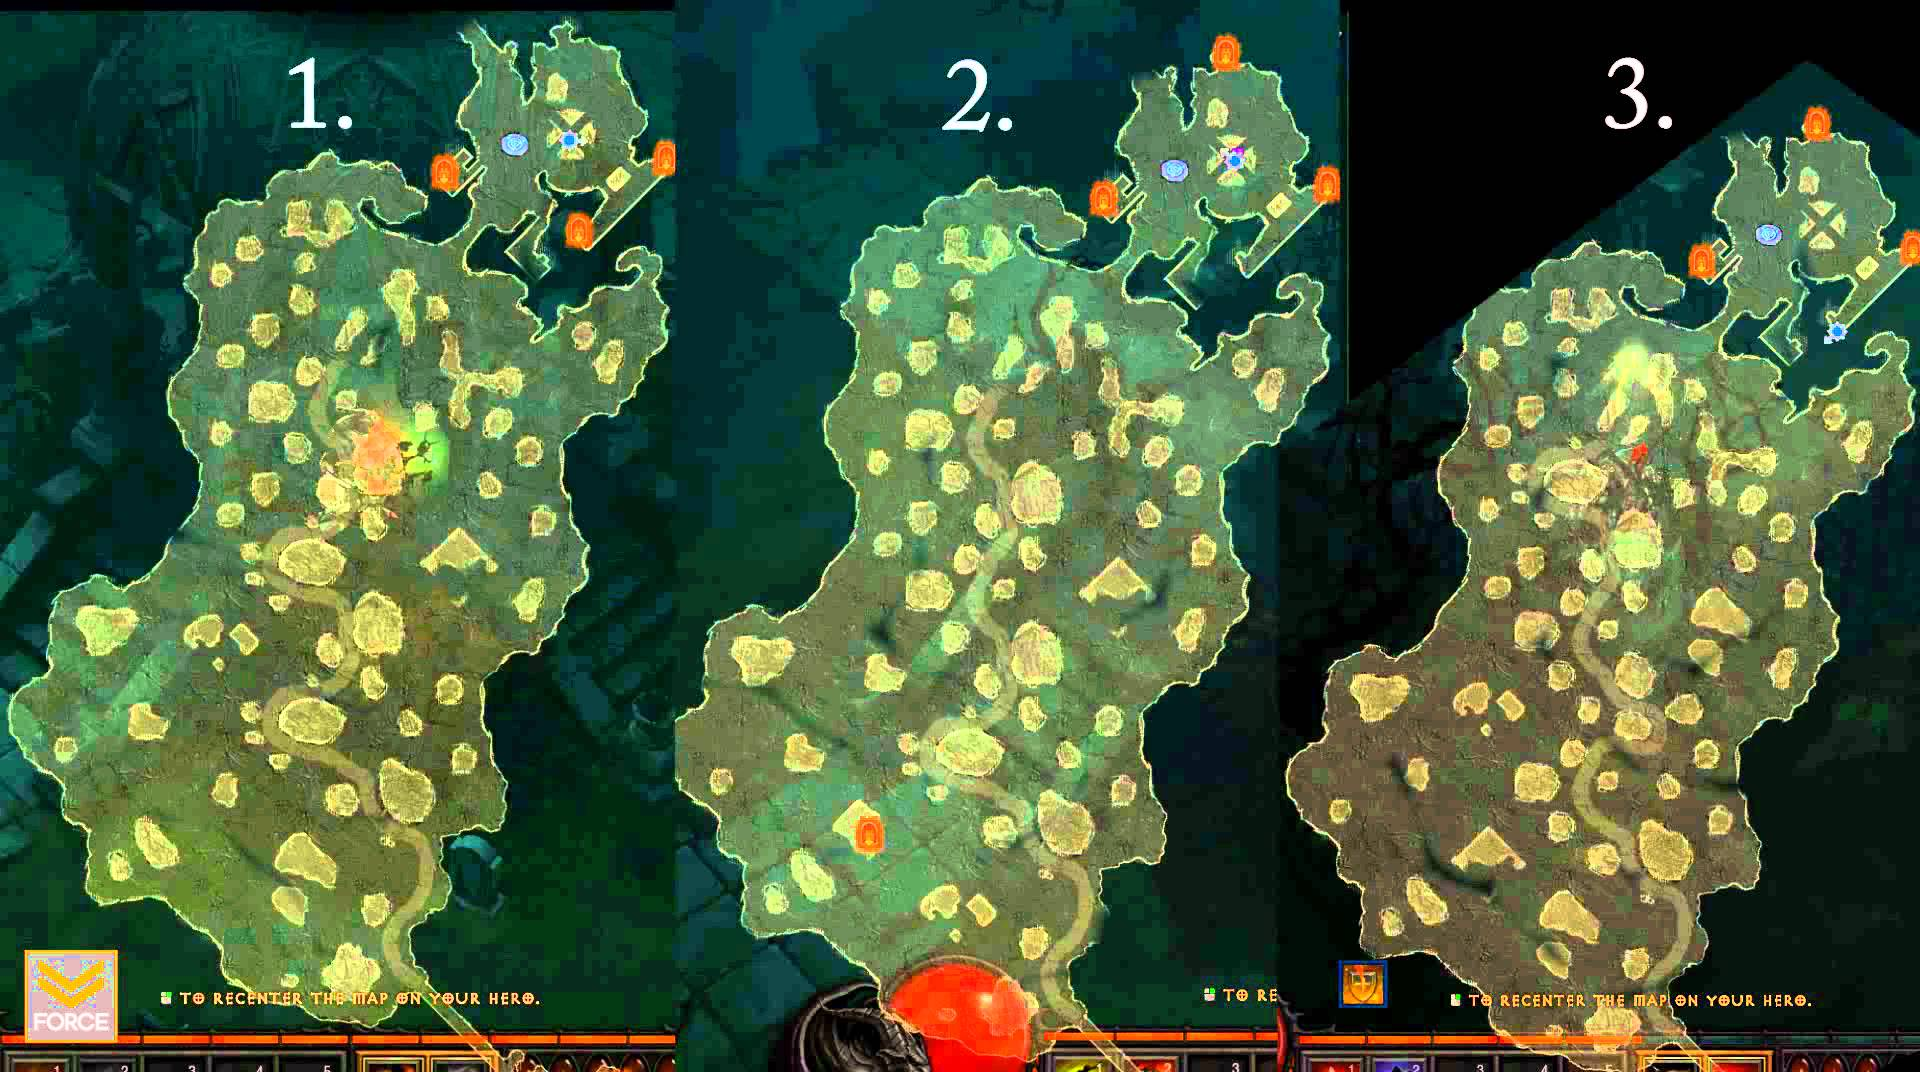
\includegraphics[height=6cm]{images/diabloMap}
	\label{fig:diablo}
\end{figure}

The diablo game world is randomly generated on runtime, which means that the map is never the same (see \autoref{fig:diablo}), Project-Y! will incorporate a feature like the random map from Diablo, where the map is randomized as the player moves around in the game world.\\
\begin{figure}[H]
	\centering
	\caption{A picture showing the viewing angle in GTA 2}
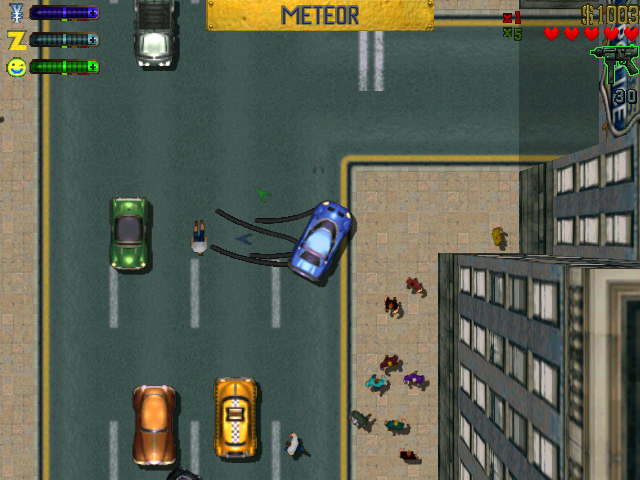
\includegraphics[height=6cm]{images/gta2.png}
	\label{fig:gta2}
\end{figure}

GTA 2 has a top down camera, where everything is seen from above (see \autoref{fig:gta2}). ProjectY! will also have a top down viewing angle, so that everything is seen from above.\\
\begin{figure}[H]
	\centering
	\caption{A picture showing the the stationary camera from Asterroids}
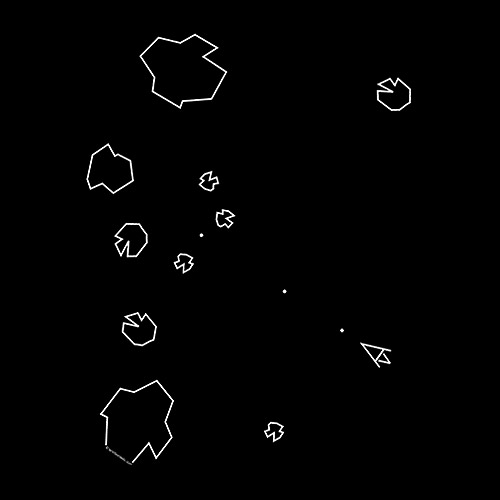
\includegraphics[width=8cm]{images/asteroids}
	\label{fig:ast}
\end{figure}
Asteroids has a stationary camera, where the camera is standing still, and all the elements are moving around, this means that the camera is not following the player, and the player can move freely. In Project-Y! the camera shall be stationary, and when the player moves out of the camera sight, a new map is generated which the player enters from the appropriate side.
\end{document}